\PassOptionsToPackage{top=3cm,left=3cm,right=3cm,bottom=3cm}{geometry}
\documentclass[fleqn,11pt]{wlscirep}

\usepackage{import}
\usepackage{main}

\renewcommand{\paragraph}[1]{\vspace{0.3cm}\noindent\underline{\emph{#1}}\hfill\noindent}

\begin{document}

\doublespacing

\title{\bfseries\LARGE\singlespacing{Molecular detection of SARS-CoV-2 and other respiratory viruses in saliva and bioaerosols}}

% author list
\author[1,2]{Nicolas Banholzer}
\author[2,3]{Philipp Jent}
\author[2,4]{Pascal Bittel}
\author[1]{Kathrin Zürcher}
\author[4]{Lavinia Furrer}
\author[1]{Simon Bertschinger}
\author[5]{Ernest Weingartner}
\author[2,4]{Alban Ramette}
\author[1,6,7]{Matthias Egger}
\author[2,8]{Tina Hascher}
\author[1*,2]{Lukas Fenner}

\affil[1]{Institute of Social and Preventive Medicine, University of Bern, Bern, Switzerland}
\affil[2]{Multidisciplinary Center for Infectious Diseases, University of Bern, Bern, Switzerland}
\affil[3]{Department of Infectious Diseases, Inselspital, Bern University Hospital, University of Bern, Bern, Switzerland}
\affil[4]{Institute for Infectious Diseases, University of Bern, Bern, Switzerland}
\affil[5]{Institute for Sensors and Electronics, University of Applied Sciences and Arts Northwestern Switzerland, Windisch, Switzerland}
\affil[6]{Population Health Sciences, University of Bristol, Bristol, UK}
\affil[7]{Centre for Infectious Disease Epidemiology and Research, University of Cape Town, Cape Town, South Africa}
\affil[8]{Institute of Educational Science, University of Bern, Bern, Switzerland}

\affil[*]{Corresponding author: lukas.fenner@unibe.ch}


\vspace{2em}

%TC:ignore

\begin{information}\normalfont
\textbf{Word count:} Abstract 219 (max 250), Manuscript 1,380 (max 1,200) \\
\textbf{Display items:} Figure 1 (max 2) \\
\textbf{References:} 15 (max 15) \\
%\textbf{Supporting information:} STROBE checklist, Supplementary Data with texts, tables, and figures
% \par
\end{information}

\begin{abstract}\normalfont
\noindent \textbf{Objectives:} To compare molecular detection of SARS-CoV-2 and other respiratory viruses in saliva and bioaerosols. 

\noindent \textbf{Methods:} We analyze saliva and bioaerosol samples from two studies conducted in winter 2021/2022 (during the SARS-CoV-2 omicron wave) and winter 2022/2023 (after the COVID-19 pandemic) in a Swiss school setting. We estimate the probability of weekly airborne detection of SARS-CoV-2 vs non-SARS-CoV-2 viruses using a Bayesian logistic regression model.

\noindent \textbf{Results:} While during the pandemic SARS-CoV-2 was almost exclusively detected in saliva (19~samples of SARS-CoV-2 vs 2~samples of non-SARS-CoV-2), the most common respiratory viruses after the pandemic were adenovirus, influenza, and rhinoviruses (3~samples of SARS-CoV-2 vs 47~samples of non-SARS-CoV-2). Despite the same study setting and methods used, airborne detection of SARS-CoV-2 was relatively more frequent than of non-SARS-CoV-2 viruses (10~samples of SARS-CoV-2 in 2021/2022 vs 2~samples of non-SARS-CoV-2 in 2022/2023). Based on our model, the posterior probability of weekly airborne detection was 31\% (95\%-credible interval [CrI] 13\%$-$54\%) for SARS-CoV-2 vs 11\% (95\%-CrI 4\%-23\%) for non-SARS-CoV-2. 

\noindent \textbf{Discussion:} There was a clear shift in the distribution of respiratory viruses from predominantely SARS-CoV-2 in 2022 to other respiratory viruses in 2023. Our comparison suggests that SARS-CoV-2 is easier to detect in the air than other endemic respiratory viruses, possibly facilitating long-range transmission. Future experimental studies are needed to confirm this finding. \medskip

\par
\end{abstract}

\flushbottom
\maketitle

\vspace{2em}

\vspace{0.5em}

\noindent\textbf{Keywords:} respiratory viruses; SARS-CoV-2; influenza; airborne transmission; molecular detection
% maximum of 3-5 keywords

\thispagestyle{empty}
\sloppy
\raggedbottom

\newpage
%TC:endignore

\setcounter{page}{1}

\section*{Introduction}

The transmission of respiratory viruses, such as SARS-CoV-2 and influenza, within schools and and other indoor environments is difficult to control\cite{Leung2020}. Respiratory viruses spread by multiple routes, including respiratory particles such as large droplets and small aerosols. Unlike larger droplets, which settle quickly, aerosols can remain suspended in the air for extended periods\cite{Wang2021}. Airborne transmission is probably significant, but the relative contribution to overall transmission is still unclear, particularly because detection of respiratory viruses in the air remains challenging\cite{Belser2023PLOSPath}.

Airborne infectious pathogens are primarily found in smaller particles (<10$\mu$m) and the distribution is similar across a range of different pathogens\cite{Fennelly2020}. Thus, pathogen-carrying aerosols have the potential for long-range transmission, but the larger concentration of particles near the infectious person favours short-range transmission\cite{Tellier2009JTRSI,Wang2020}. The complexity of airborne transmission lies in the interplay between the physicochemical properties of pathogen-carrying aerosols and environmental conditions\cite{Wang2021}, making it challenging to devise effective public health strategies to mitigate the spread of respiratory infections in various indoor settings, including schools, offices, and hospitals.

In this study, we compared saliva samples, bioaerosol samples, and samples from the HEPA filters of air cleaners that were collected as part of two studies that we conducted in a Swiss school setting in winter 2021/2022 (during the SARS-CoV-2 omicron wave, henceforth 2022)\cite{Banholzer2023PLoSMed} and winter 2022/2023 (after the COVID-19 pandemic, henceforth 2023)\cite{Banholzer2023submitted}. We show differences in the distribution of respiratory viruses and analyze the results from airborne molecular detection. 


\section*{Methods}

Data was collected in two Swiss secondary schools (age of students 14-17~years) in the canton of Solothurn, Switzerland, over a seven-week study period from end of January to beginning of March. Three classes participated in 2022 and two classes in 2023. Two classes shared the same classroom in 2022 due to half-class teaching, other classes had a separate classroom. All classrooms were not equipped with an active HVAC (heating, ventilation, air conditioning) system, but were ventilated using passive window ventilation. An air quality device (AQ Guard, Palas GmbH, Karlsruhe, Germany) continuously measured indoor CO$_2$ levels, temperature, and humidity. A detailed comparison of the study settings can be found in \supp~Table~\zref{tab:comp_study}. 

Repetitive testing for a panel of respiratory infections was done weekly in 2022 and bi-weekly in 2023. Airborne respiratory viruses were collected in each classroom with a cyclonic bioaerosol sampling device (Coriolis Micro Air, Bertin Instruments Montigny-le-Bretonneux, France) and a BioSpot-VIVAS condensation particle growth collection device (Aerosol Devices Inc., Ft. Collins, CO, USA)\cite{Lednicky2016AST}. The removable parts were regularly autoclaved. Finally, swabs from the air cleaners' HEPA filters were collected. The HEPA filters were removed and divided into 20~fields. One sterile Phosphate-Buffered Saline-moistened swab per field was then taken for a total of 20~swabs per filter. Saliva and airborne samples were transported to the Institute of Infectious Diseases and stored at $-$80°C until further processing\cite{Huber2021}. Prior to the real-time (RT)-PCR analysis, daily bioaerosol samples were combined for each sampling device and filtered using Amicon Ultra-15 Centrifugal Filters with Ultracel 10,000 Dalton molecular weight cutoffs filters (UFC9010; MilliporeSigma, Burlington, USA) to a volume of 1\,mL. Saliva samples were analyzed directly without prior filtration. The Allplex RV Master Assay (Seegene, Seoul, South Korea) detects a panel of 19 major respiratory viruses and viral subtypes, including SARS-CoV-2, influenza A/B, respiratory syncytial, metapneumovirus, adenovirus, rhinovirus, and parainfluenza. 

Descriptive statistics were used to present differences in the type and number of respiratory viruses detected in saliva and airborne samples between 2022 and 2023. A Bayesian logistic regression model was used to estimate the probability of detecting any SARS-CoV-2 vs non-SARS-CoV-2 in the air during a study week, adjusting for differences in the study settings and the interventions that were in place during the studies (see \supp~Text~\zref{sec:model} for a detailed model description).   

\section*{Results}

In 2022, 58~students participated in weekly saliva testing. There were 21~positive saliva samples over the study, namely 19~SARS-CoV-2, 1~influenza~A, and 1~adenovirus (\Cref{fig:comparison}a, left). There were 10~positive bioaerosol samples, namely 9~SARS-CoV-2 and 1~adenovirus. There were 8~positive samples on the HEPA-filters of the air cleaners, namely 6~SARS-CoV-2, 1~influenza~A and 1~adenovirus. In 2023, 38~students participated in bi-weekly saliva testing. There were 50~positive saliva samples over the study, namely 15~influenza~B, 15~rhinovirus, 14~adenovirus, 3~SARS-CoV-2, 2~metapneumovirus, 1~parainfluenza virus (\Cref{fig:comparison}a, right). There were 2~positive bioaerosol samples, namely 1~rhinovirus and 1~adenovirus. There were 4~positive samples on the HEPA-filters of the air cleaners, namely 1~influenza~B, 1~rhinovirus, 1~adenovirus, and 1~SARS-CoV-2. 

We found 6 positive air-saliva samples in the same respective week (4~SARS-CoV-2 and 2~non-SARS-CoV-2 (\Cref{fig:comparison}b), suggesting they were paired samples. Based on our Bayesian logistic regression model, SARS-CoV-2 was more likely detected in bioaerosols than non-SARS-CoV-2 (adjusted odds ratio 3.6, 95\%-CrI 1.5$-$8.9). The probability of molecular airborne detection was 31\% (95\%-credible interval [CrI] 13\%$-$54\%) for SARS-CoV-2 vs 11\% (95\%-CrI 4\%-23\%) for non-SARS-CoV-2 (\Cref{fig:comparison}c). Our estimates are adjusted for differences in the daily maximum CO$_2$ level, which was 1,134\,ppm (standard deviation [SD] 277\,pppm) in 2022 compared to 2,224\,ppm (SD 321\,pppm) in 2023. Humidity and temperature were similar, with daily mean relative humidity of 38\% (SD 6\%) in 2022 vs 38\% (SD 5\%) in 2023 and daily mean temperature of 19°C (SD 2°C) in 2022 vs 22°C (SD 1°C) in 2023. 

\begin{figure}
    \centering
    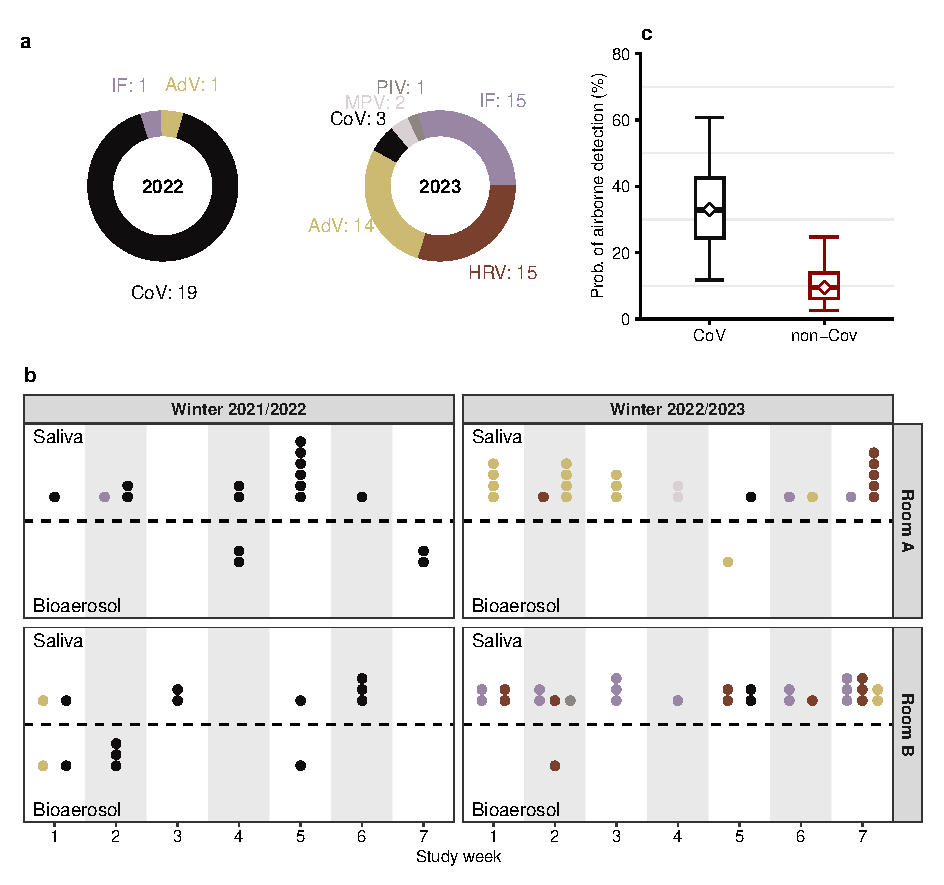
\includegraphics{results/comparison.pdf}
    \caption{Comparison of molecular detection of respiratory viruses between winter 2021/2022 (2022) and winter 2022/2023 (2023). \textbf{(a)}~Distribution of respiratory viruses found in saliva. IF: influenza~A/B, HRV: human rhinovirus, AdV: adenovirus, CoV: SARS-CoV-2, MPV: human metapneumovirus, PIV: parainfluenza virus. \textbf{(b)}~Positive samples in saliva and bioaerosols per study week. \textbf{(c)}~Probability of detecting any SARS-CoV-2 and non-SARS-CoV-2 in bioaerosols during a study week (posterior mean as dots, interquartile range as box, 95\%-CrI as error bars).}
    \label{fig:comparison}
\end{figure}


\section*{Discussion}

% In comparison, 

We compared molecular data collected from two studies in Swiss secondary schools in winter 2021/2022 (2022) and 2022/2023 (2023). We detected predominantly SARS-CoV-2 in 2022 and predominantly non-SARS-CoV-2 viruses, such as influenza and adenovirus, in 2023. Molecular airborne detection of SARS-CoV-2 was more likely than of non-SARS-CoV-2.

The differences between the two study periods (pandemic versus non-pandemic) suggest that SARS-CoV-2 is easier to detect in the air. One possible explanation is that SARS-CoV-2 can remain suspended and active in the air for extended periods of time, facilitating long-range transmission. In contrast, non-SARS-CoV-2 viruses were rarely detected in the air, suggesting they settle or become inactive more quickly. Therefore, prolonged close contact may be relatively more important for the transmission of respiratory viruses other than SARS-CoV-2, although previous studies suggest it also facilitates the transmission of SARS-CoV-2\cite{Leung2020NatMed,Lind2023NatCommun}.

Technical reasons for the differences in airborne detection are unlikely because the bioaerosol sampling devices and laboratory procedures were the same in both studies, and no technical problems were observed. Temperature and relative humidity were also similar in both study periods, but the same levels may have virus-specific effects on airborne survival\cite{Tellier2009JTRSI,Davis1971AM}. Ventilation changed profoundly, but CO$_2$ levels were even higher in 2023, possibly enhancing airborne survival. Additional differences in the study setting (\supp~Table~\zref
{tab:comp_study}) that could have influenced airborne detection were adjusted for in the Bayesian model (\supp~Text~\zref{sec:model}). Therefore, we speculate that the difference in airborne detection is due to the different characteristics of the respiratory viruses which can influence the generation and survival of airborne viral RNA\cite{Wang2021}. Low viral loads do often not exceed the detection limits of existing devices for bioaerosol sampling. For example, one study failed to detect any human rhinovirus in the exhaled breath of 16~HRV-infected subjects\cite{Fabian2011JAMPDD}. Finally, the ability to detect pathogens in bioaerosols may be related to the variation in infectiousness between study participants, which is associated with the generation of pathogenic aerosols\cite{Leung2020NatMed,Bischoff2013JID}. 

In conclusion, we observed a clear shift in the distribution of respiratory viruses from predominantly SARS-CoV-2 in 2022 to predominantly non-SARS-CoV-2 viruses in 2023. Molecular airborne detection of SARS-CoV-2 was more likely than of other endemic respiratory viruses, but future experimental studies are needed to confirm this finding.   


\bibliography{references.bib}

\end{document}